\chapter{Error Analysis}
\label{cha:Error Analysis}
In this chapter, in an attempt to determine the limitation of the model trained on the standard training objective and improvements that hybrid training brings to relation prediction, we will mainly study the best models trained on hybrid and standard training objectives only. The models that we examined are from the unrestricted HPC space. We note that semi-unrestricted HPC space yielded better models; however, we have not fully explored that HPC space. Therefore, future work should concentrate on that HPC space.

Additionally, we only examine the best models selected based on entity MRR and overall MRR. Those two model selection methods are chosen because we can find the best performance on relation and entity prediction using those two. We could not ignore the importance of entity prediction, although the thesis is about relation prediction. 

For simplicity, the \textit{"standard model"} is used to refer to a model trained on a standard training objective. The best standard model which is selected based on entity MRR will be referred to as the \textit{"standard entity model}. "Next, the best standard model selected on overall MRR will be called as \textit{"standard overall model"}. In this chapter, the standard entity model is our \textit{"baseline model"}.

If a model is trained on a hybrid training objective, we will refer them to a \textit{hybrid model}. The \textit{hybrid entity model} will be referred to as the best hybrid model selected on entity MRR and the \textit{hybrid overall model} is used to name the best hybrid model selected on overall MRR. 

Within this chapter, the FB15K-237 dataset is used to perform the error analysis. We chose this particular HPC space because we observed the improvement when applying the hybrid training objective. 

\section{Standard entity model and its limitation}

To reveal the limitations of baseline model (i.e., standard entity model) on relation prediction task, we attempted to calculate the relation MRR for each relation. More precisely, for a specific relation $k$, we extracted all triples in a validation data $\mathcal{V}$ (or training data $\mathcal{T}$) that are formed by that relation $k$ i.e., $$\mathcal{D}_{j,\mathcal{V}} = \{(i,k,j) | i,j \in \mathcal{E} \vee (i,k,j) \in \mathcal{V} \}$$ or $$\mathcal{D}_{k,\mathcal{T}} = \{(i,k,j) | i,j \in \mathcal{E} \vee (i,k,j) \in \mathcal{T} \}$$. Then we calculated the filtered relation MRR for that relation $k$ based on all of those triples in set $\mathcal{D}_{k,\mathcal{V}}$ (or $\mathcal{D}_{k,\mathcal{T}}$). Formally, for example, the relation MRR for that relation $k$ on validation data will be calculated by using this formula:
\begin{equation}
 \begin{split}
    \text{Filtered MRR}_{\text{relation, } j,\mathcal{V}} =
    \frac{1}{|\mathcal{D}_{j,\mathcal{V}}|}
    \sum_{(i,k,j)\in\mathcal{D}_{j,\mathcal{V}}}  
    \bigg(
    & \frac{1}{\text{rank}(k|i,j)} \bigg) 
\end{split}
\end{equation}
We performed the calculation in validation and training data independently. 

In their paper, \citet{chang2020benchmark} suggested analyzing the model performance in each relation type  (i.e., M-M, M-1, 1-N, and 1-1). The main difference between those four types is the number of entities that a subject or an object can associate with. For example, the basic difference between M-N and M-1 relation types is the number of objects that a subject can associate with, e.g., M-N relation - "lived place" and M-1 relation - "place of birth". A person can live in more than one place, however, there is only one birthplace for a person. Figure \ref{fig:RelationMRR boxplot} shows the distribution of filtered relation MRRs for each relation type and model.

\begin{figure}[!htbp]
	\begin{center}
	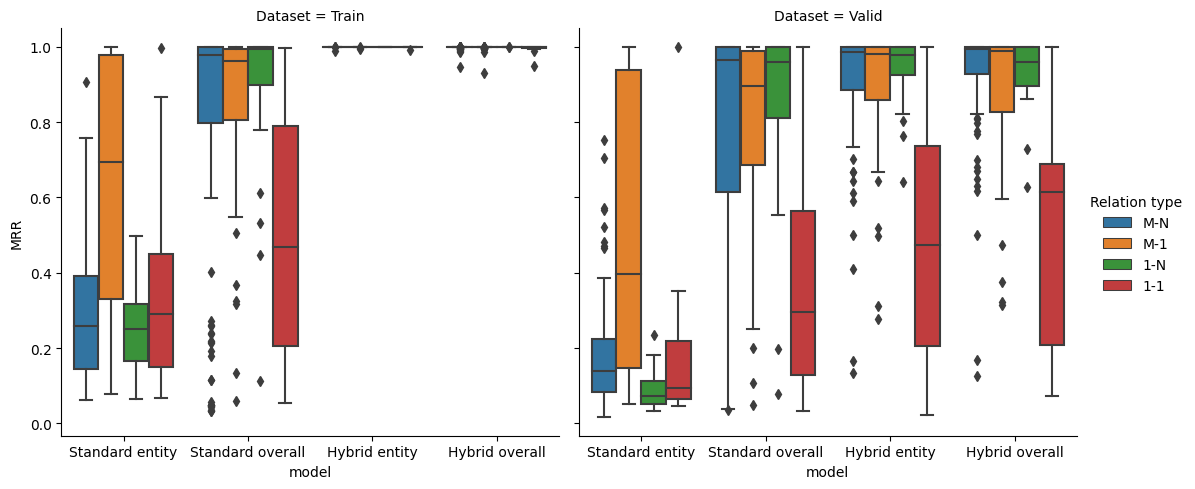
\includegraphics[width=1.0\linewidth]{Images/RelationMRR_boxplot.png}
	\caption[Distribution of filtered relation MRR]{Distribution of filtered relation MRR on validation and training data over relations for four relation types (M-M, M-1, 1-N, and 1-1).}
	\label{fig:RelationMRR boxplot}
	\end{center}
\end{figure}


Unexpectedly, from Figure \ref{fig:RelationMRR boxplot} we can see that the standard entity model showed a wide dispersion in M-1 relations in which the the third quartile MRR is 97.9\% and the first quartitle MRR is 33.0\% in training dataset. However, for the remain types, the baseline model could achieve low MRRs i.e., the median of M-N, 1-N, and 1-1 distributions are 25.8\%, 25.0\%, and 29.0\% respectively in training dataset. Undoubtedly, we also observed the wide dispersion in M-1 relation and low medians in M-N, 1-N, and 1-1 the relations on validation data. Those findings indicates that the model seems to be biased toward the M-1 relations. Therefore, it is necessary to observe the common ranking patterns which the baseline model ranked in four relation types (i.e., M-M, M-1, 1-N, and 1-1).

Table \ref{tab:Top 3 predictions for each relation type} shows the top three ranking patterns as well as their percentage. The ranking pattern is a tuple of the relation types from top three ranked relations; for example, the (M-1, 1-1, 1-N) pattern means that the first rank relation is M-1 relation, then the second rank relation is 1-1 relation, and third rank relation is 1-N relation.  

\begin{table}[!htbp]
\centering
\resizebox{\textwidth}{!}} & \multicolumn{1}{c}{\textbf{}} & \multicolumn{1}{c}{\textbf{Top 3}} & \multicolumn{1}{c}{\textbf{\%}} & \multicolumn{1}{c}{\textbf{}} & \multicolumn{1}{c}{\textbf{Top 3}} & \multicolumn{1}{c}{\textbf{\%}} & \multicolumn{1}{c}{\textbf{}} & \multicolumn{1}{c}{\textbf{Top 3}} & \multicolumn{1}{c}{\textbf{\%}} \\ \midrule
(M-1, M-1, M-1) & 34.71 &  & (M-1, M-1, M-1) & 63.00 &  & (M-1, M-1, M-1) & 33.96 &  & (1-1, 1-1, 1-1) & 65.74 \\
(1-1, 1-1, 1-1) & 14.65 &  & (M-1, M-1, 1-N) & 7.97 &  & (M-1, M-1, 1-N) & 10.52 &  & (M-1, 1-1, 1-1) & 8.71 \\
(M-1, M-1, M-N) & 5.59 &  & (M-1, 1-N, M-1) & 7.35 &  & (M-1, 1-N, M-1) & 6.97 &  & (1-1, M-1, 1-1) & 5.33 \\ \bottomrule
\end{tabular}%
}
\caption{Three top-3 predictions for each relation type (training)}
\label{tab:Top 3 predictions for each relation type}
\end{table}
   

Table \ref{tab:Top 3 predictions for each relation type} strongly underlines the bias of model toward the M-1 relations. The M-1 relations are, most of the time, on the top of ranking regardless of the relation type of the true relation (except 1-1 relation type). For instance, if the actual relation is a M-N relation, there is a 34.71\% chance that we observed the first, second, and third rank relations being M-1 relations. Same for if the actual relation is 1-N relation, there is 33.96\% that we observed the first, second, and third rank relations being all M-1 relations. 
% Surprisingly, the baseline model could not capture the relation types while other models could capture them and rank those relations which have the same type as actual relations higher than those are not the same type.
Table \ref{tab:standard entity model examples} shows three examples of ranking results from baseline model.  

\begin{table}[!htbp]
\centering
\resizebox{\textwidth}{!}{%
\begin{tabular}{@{}lllcc@{}}
\toprule
\textbf{Subject} & \textbf{Relation} & \textbf{Object} & \textbf{Rank} & \textbf{Type} \\ \midrule
\multirow{4}{*}{Joe Hisaishi} & /people/person/places\_lived./people/place\_lived/location & \multirow{4}{*}{\begin{tabular}[c]{@{}l@{}}Nagano \\ Prefecture\end{tabular}} & 6 & M-N \\
 & \quad /people/person/place\_of\_birth &  & 1 & M-1 \\
 & \quad /time/event/instance\_of\_recurring\_event &  & 2 & M-1 \\
 & \quad /education/educational\_institution/campuses &  & 3 & 1-1 \\ \midrule
\multirow{4}{*}{Arnold Schoenberg} & /people/person/places\_lived./people/place\_lived/location & \multirow{4}{*}{Vienna} & 8 & M-N \\
 & \quad /people/person/place\_of\_birth &  & 1 & M-1 \\
 & \quad /people/deceased\_person/place\_of\_death &  & 2 & M-1 \\
 & \quad /base/biblioness/bibs\_location/country &  & 3 & M-1 \\ \midrule
\multirow{4}{*}{\begin{tabular}[c]{@{}l@{}}Cancer \\ (Disease or \\ medical condition)\end{tabular}} & /people/cause\_of\_death/people & \multirow{4}{*}{\begin{tabular}[c]{@{}l@{}}Laurence \\ Olivier\end{tabular}} & 12 & 1-N \\
 & \quad /base/schemastaging/person\_extra/net\_worth./measurement\_unit/dated\_money\_value/currency &  & 1 & M-1 \\
 & \quad /film/person\_or\_entity\_appearing\_in\_film/films./film/personal\_film\_appearance/type\_of\_appearance &  & 2 & M-1 \\
 & \quad /film/film/estimated\_budget./measurement\_unit/dated\_money\_value/currency &  & 3 & M-1 \\ \bottomrule
\end{tabular}%
}
\caption[Prediction examples from standard entity model.]{Prediction examples from standard entity model. The first relations on the top of each box are the true relations while the remain ones are the predicted relation. \textit{Joe Hisaishi was born in Nagono and Arnold Schoenberg was also born in Veinna, however, those information was not captured in FB15K-237, so those triples are considered to be negative triples in this study.}}
\label{tab:standard entity model examples}
\end{table}




Through this example, we note that there exists some relations that share the same object and/or objects domain together. For instance, the subject for "lived places" and "place of birth" relations is the set of name of people, while their set of object is the set of cities or places. Those domain-sharing relations could be considered as hard-cases for relation predictions. 

Formally, a \textit{domain-sharing relations} is a relations such that there exists another relation(s) in knowledge graph which share the same subject and object; for example, Mr.A lived in Ha Noi and Mr.A was born in Ha Noi. On the other hand, \textit{non domain-sharing relations} are those relations which do not have relation sharing the same subject and object in data. In FB15k-237, there are totally 160 domain-sharing relations which takes about 67.5\% total relations in dataset. However, there are only 29160 triples which are formed from 160 domain-sharing relations, those triples take 10\% of total triple in the training dataset. Those triples could be considered as the corner-cases. 

Figure \ref{fig:MRR relation in so pairs (standard entity)} shows the distributions of filtered relation MRRs for domain-sharing and non domain-sharing relations on validation and training dataset. Perhaps unsurprisingly, we found from Figure \ref{fig:MRR relation in so pairs (standard entity)} that baseline mode tends to perform better on non domain-sharing relations than on domain-sharing relations. The median MRRs of non domain-sharing relation are always higher than median MRRs of domain-sharing relation. 

\begin{figure}[!htbp]
	\begin{center}
	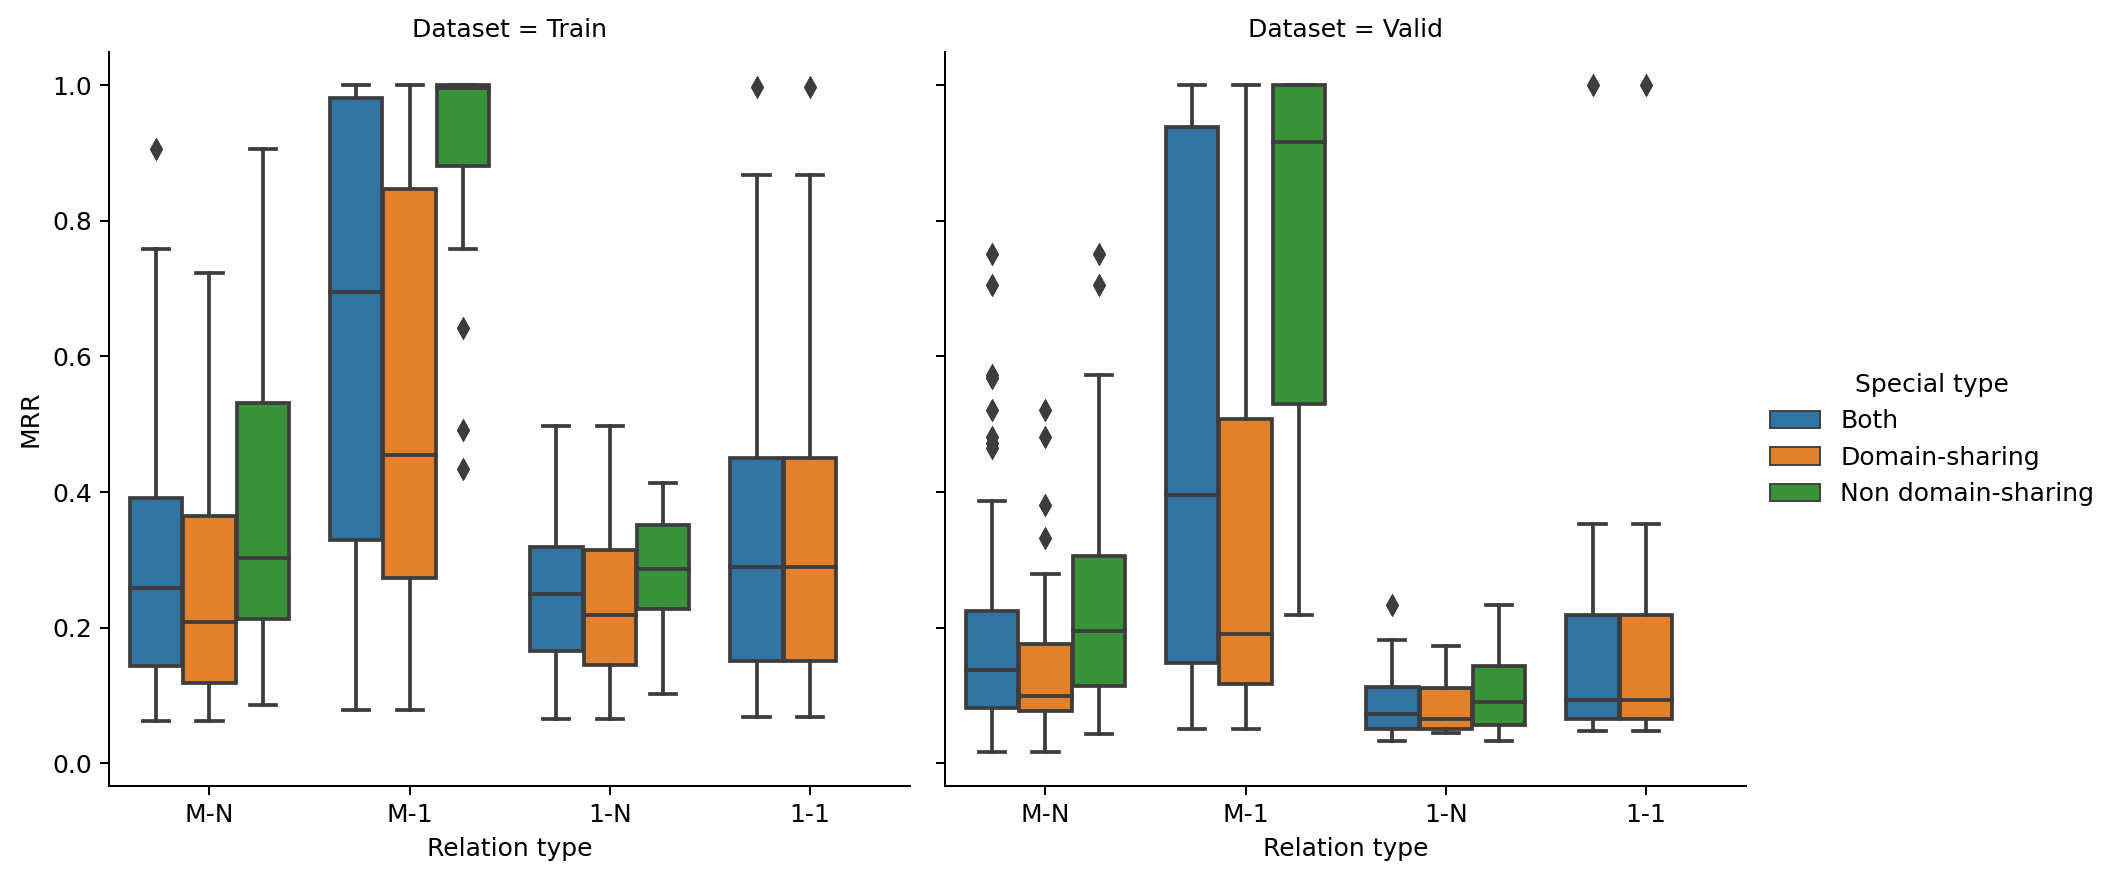
\includegraphics[width=\linewidth]{Images/MRR_relation_in_so_pairs (standard entity).png}
	\caption[Distribution of filtered relation MRR (standard entity)]{Distribution of filtered relation MRR on validation and training data over relations for for non domain-sharing and domain-sharing relations (standard entity model)}
	\label{fig:MRR relation in so pairs (standard entity)}
	\end{center}
\end{figure}

We attempt to measure the similarity between the top-rank relation $k'$ and the actual relation $k$ based on domain similarity. To do so, we calculated the Jaccard similarity between (1) the subject sets between those two relation and between the object sets of those two relations. Then the similarity between two relation is the average of subject and object Jaccard similarities. The set of subjects (or objects) of a relation $\mathcal{E}_{s, k'}$ (or $\mathcal{E}_{o, k'}$) is defined as $\mathcal{E}_{s, k'} = \{i'|i'\in\mathcal{E} \vee (i',k',*) \in \mathcal{T}\}$ (or $\mathcal{E}_{o, k'} = \{j'|j'\in\mathcal{E} \vee (*,k',j') \in \mathcal{T}\}$), where $\mathcal{T}$ is the training dataset. Thus, the similarity between two sets of subject, for example, is calculated using this formula $$J(\mathcal{E}_{s, k},\mathcal{E}_{s, k'}) = \frac{|\mathcal{E}_{s, k} \cap \mathcal{E}_{s, k'}|}{|\mathcal{E}_{s, k} \cup \mathcal{E}_{s, k'}|}$$. 

\begin{figure}[!htbp]
	\begin{center}
	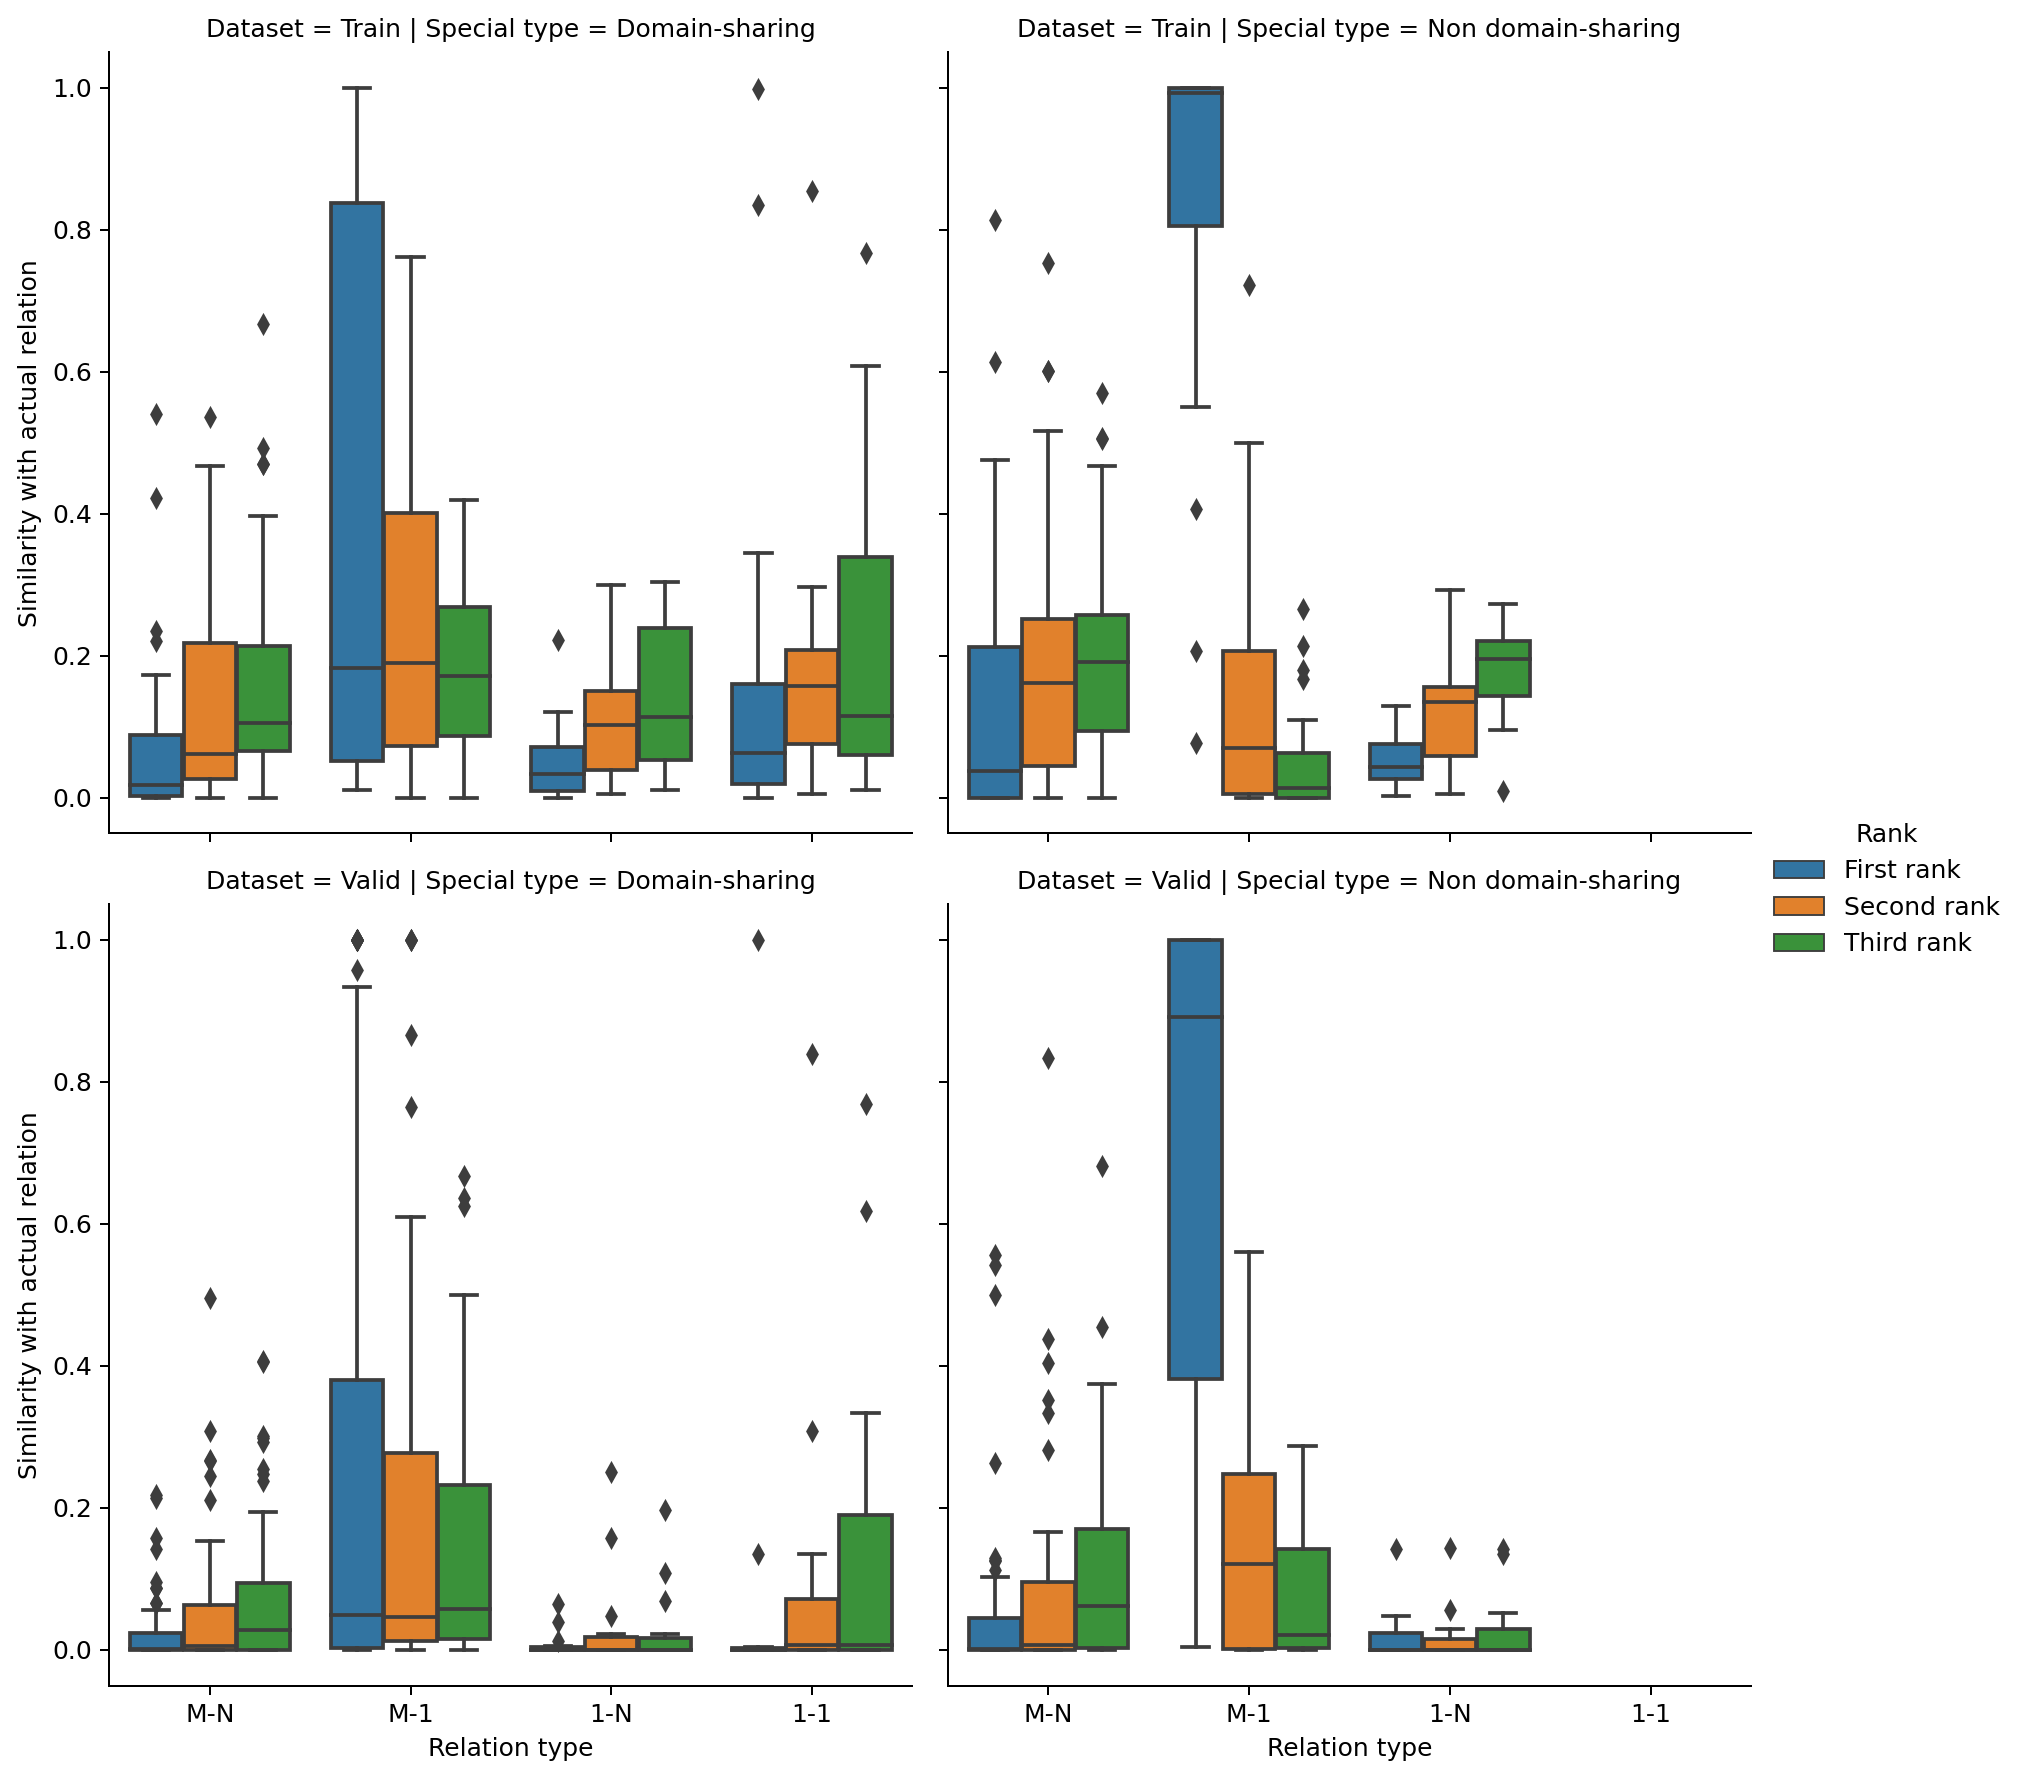
\includegraphics[width=\linewidth]{Images/jaccard_similarity (standard entity).png}
	\caption[Distribution of average similarity (standard entity)]{Distribution of average similarity between ranked relation and actual relation on validation and training data over relations for non domain-sharing and domain-sharing relations (standard entity model)}
	\label{fig:Jaccard similarity (standard entity)}
	\end{center}
\end{figure}

The Figure \ref{fig:Jaccard similarity (standard entity)} shows the the distribution of average similarity between ranked relation and actual relation for domain-sharing relations and non domain-sharing relations.
Predictably, the top-rank relations are not similar to actual relation in term of domain similarity except M-1 relation type. There are, however, some interesting finding across relation types. We found that baseline model could rank relations which are similar to the actual relation higher for non domain-sharing relation, especially for M-1 relations, while, for domain-sharing relations, the similarity between high-rank relations and the corresponding actual relations are lower. Furthermore, the distribution of similarity for M-1 relations are more dispersed.

In sum, based on observation in Figure \ref{fig:Jaccard similarity (standard entity)} and \ref{fig:MRR relation in so pairs (standard entity)}, we found that baseline model could not capture the domain similarity, especially domain similarity of domain-sharing relations and the model tends to rank M-1 relations higher than other types regrading the type of actual relation. 

\section{Improvements from selecting on overall MRR}

As was mentioned in the Section \ref{sec:Training objectives}, without training from scratch, we can obtain a better standard model for relation prediction if we select the best-performance model base on overall MRR instead of entity MRR with a small trade-off (i.e., the entity performance of model is dropped by around 2.0\% MRR - Table \ref{tab:ICLR RP on ER vs Hybrid}). 


\begin{figure}[!htbp]
	\begin{center}
	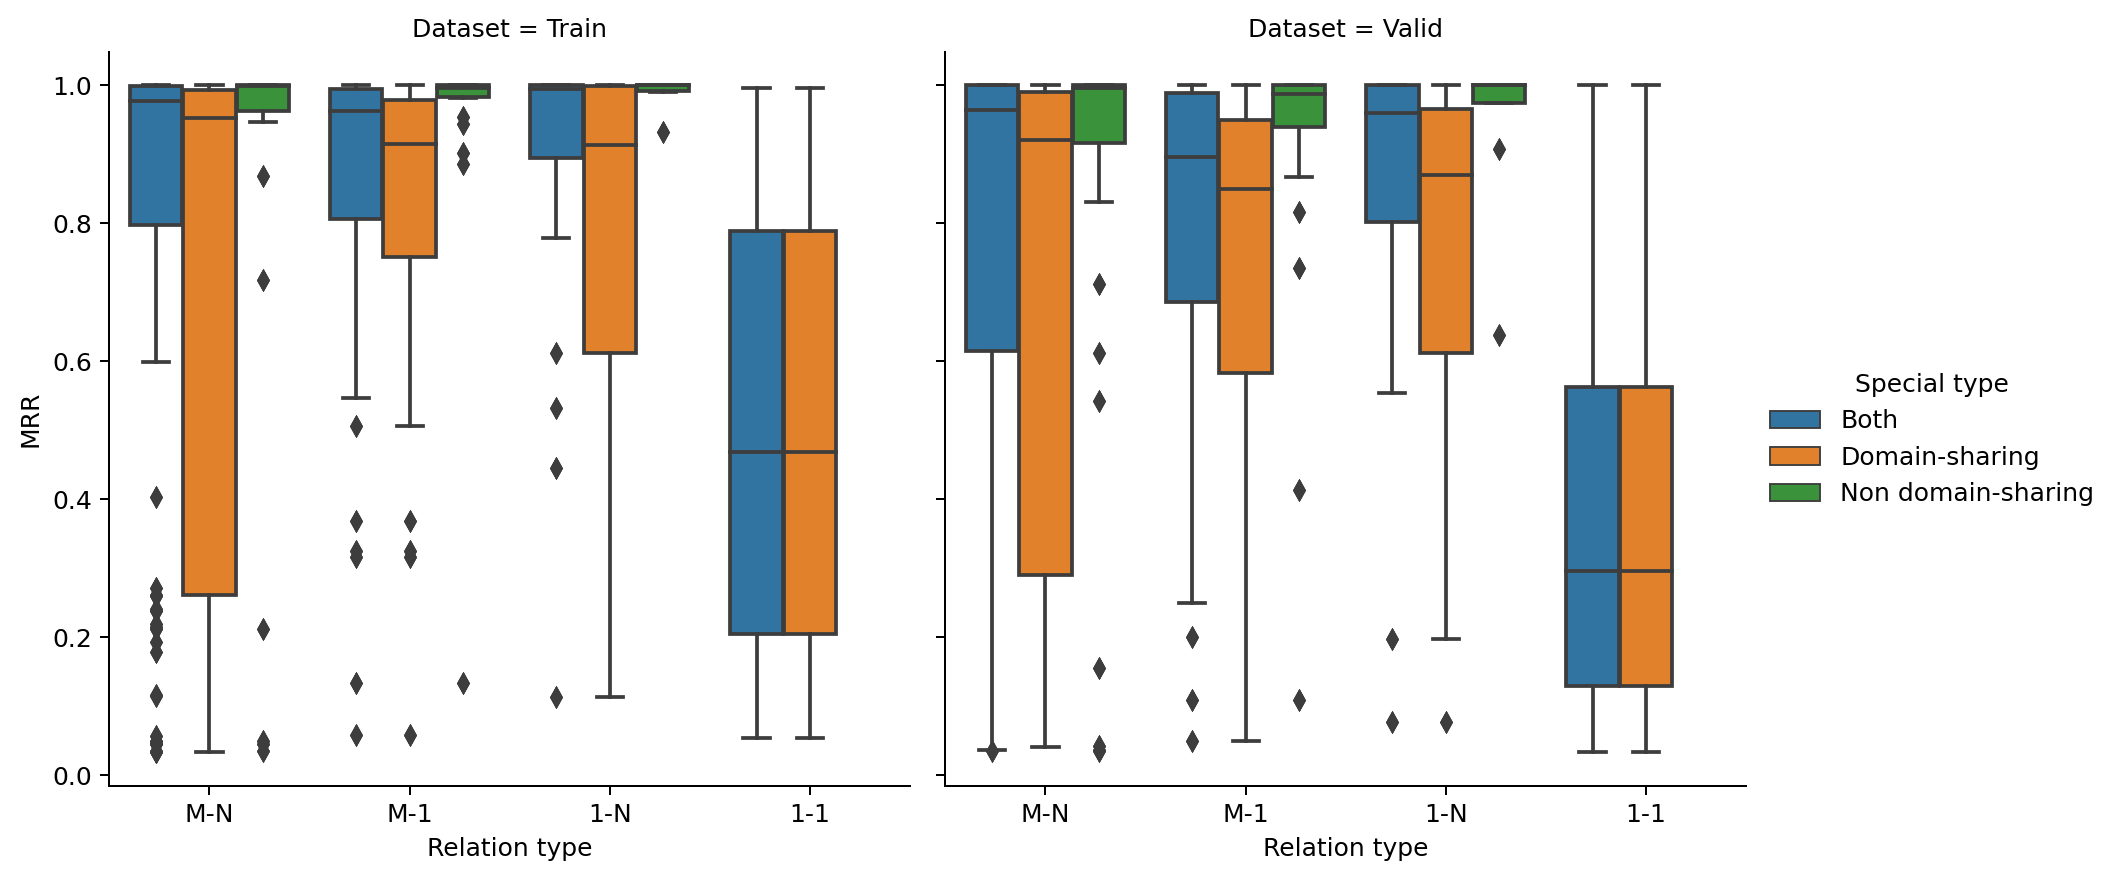
\includegraphics[width=\linewidth]{Images/MRR_relation_in_so_pairs (standard overall).png}
	\caption[Distribution of filtered relation MRR (standard overall)]{Distribution of filtered relation MRR on validation and training data over relations for for non domain-sharing and domain-sharing relations (standard overall model)}
	\label{fig:MRR relation in so pairs (standard overall)}
	\end{center}
\end{figure}

The improvement on relation prediction is illustrate nicely in Figure \ref{fig:MRR relation in so pairs (standard overall)}. As shown in that Figure, all median MRRs of standard overall model are much higher than all median MRRs of standard entity model, specially for M-N and 1-N relations on both dataset. However, the median MRRs of non domain-sharing relations still tend to be more higher than median MRRs of domain-sharing for all all relation types, and the MRR distribution of domain-sharing relations in all relation type are more dispersed compared to standard entity model. Those observations indicate that the standard overall model could achieve better MRR for most of non domain-sharing relations but only for some of domain-sharing relations. Figure \ref{fig:Jaccard similarity (standard overall)} also nicely illustrates evidences to support this claims.

\begin{figure}[!htbp]
	\begin{center}
	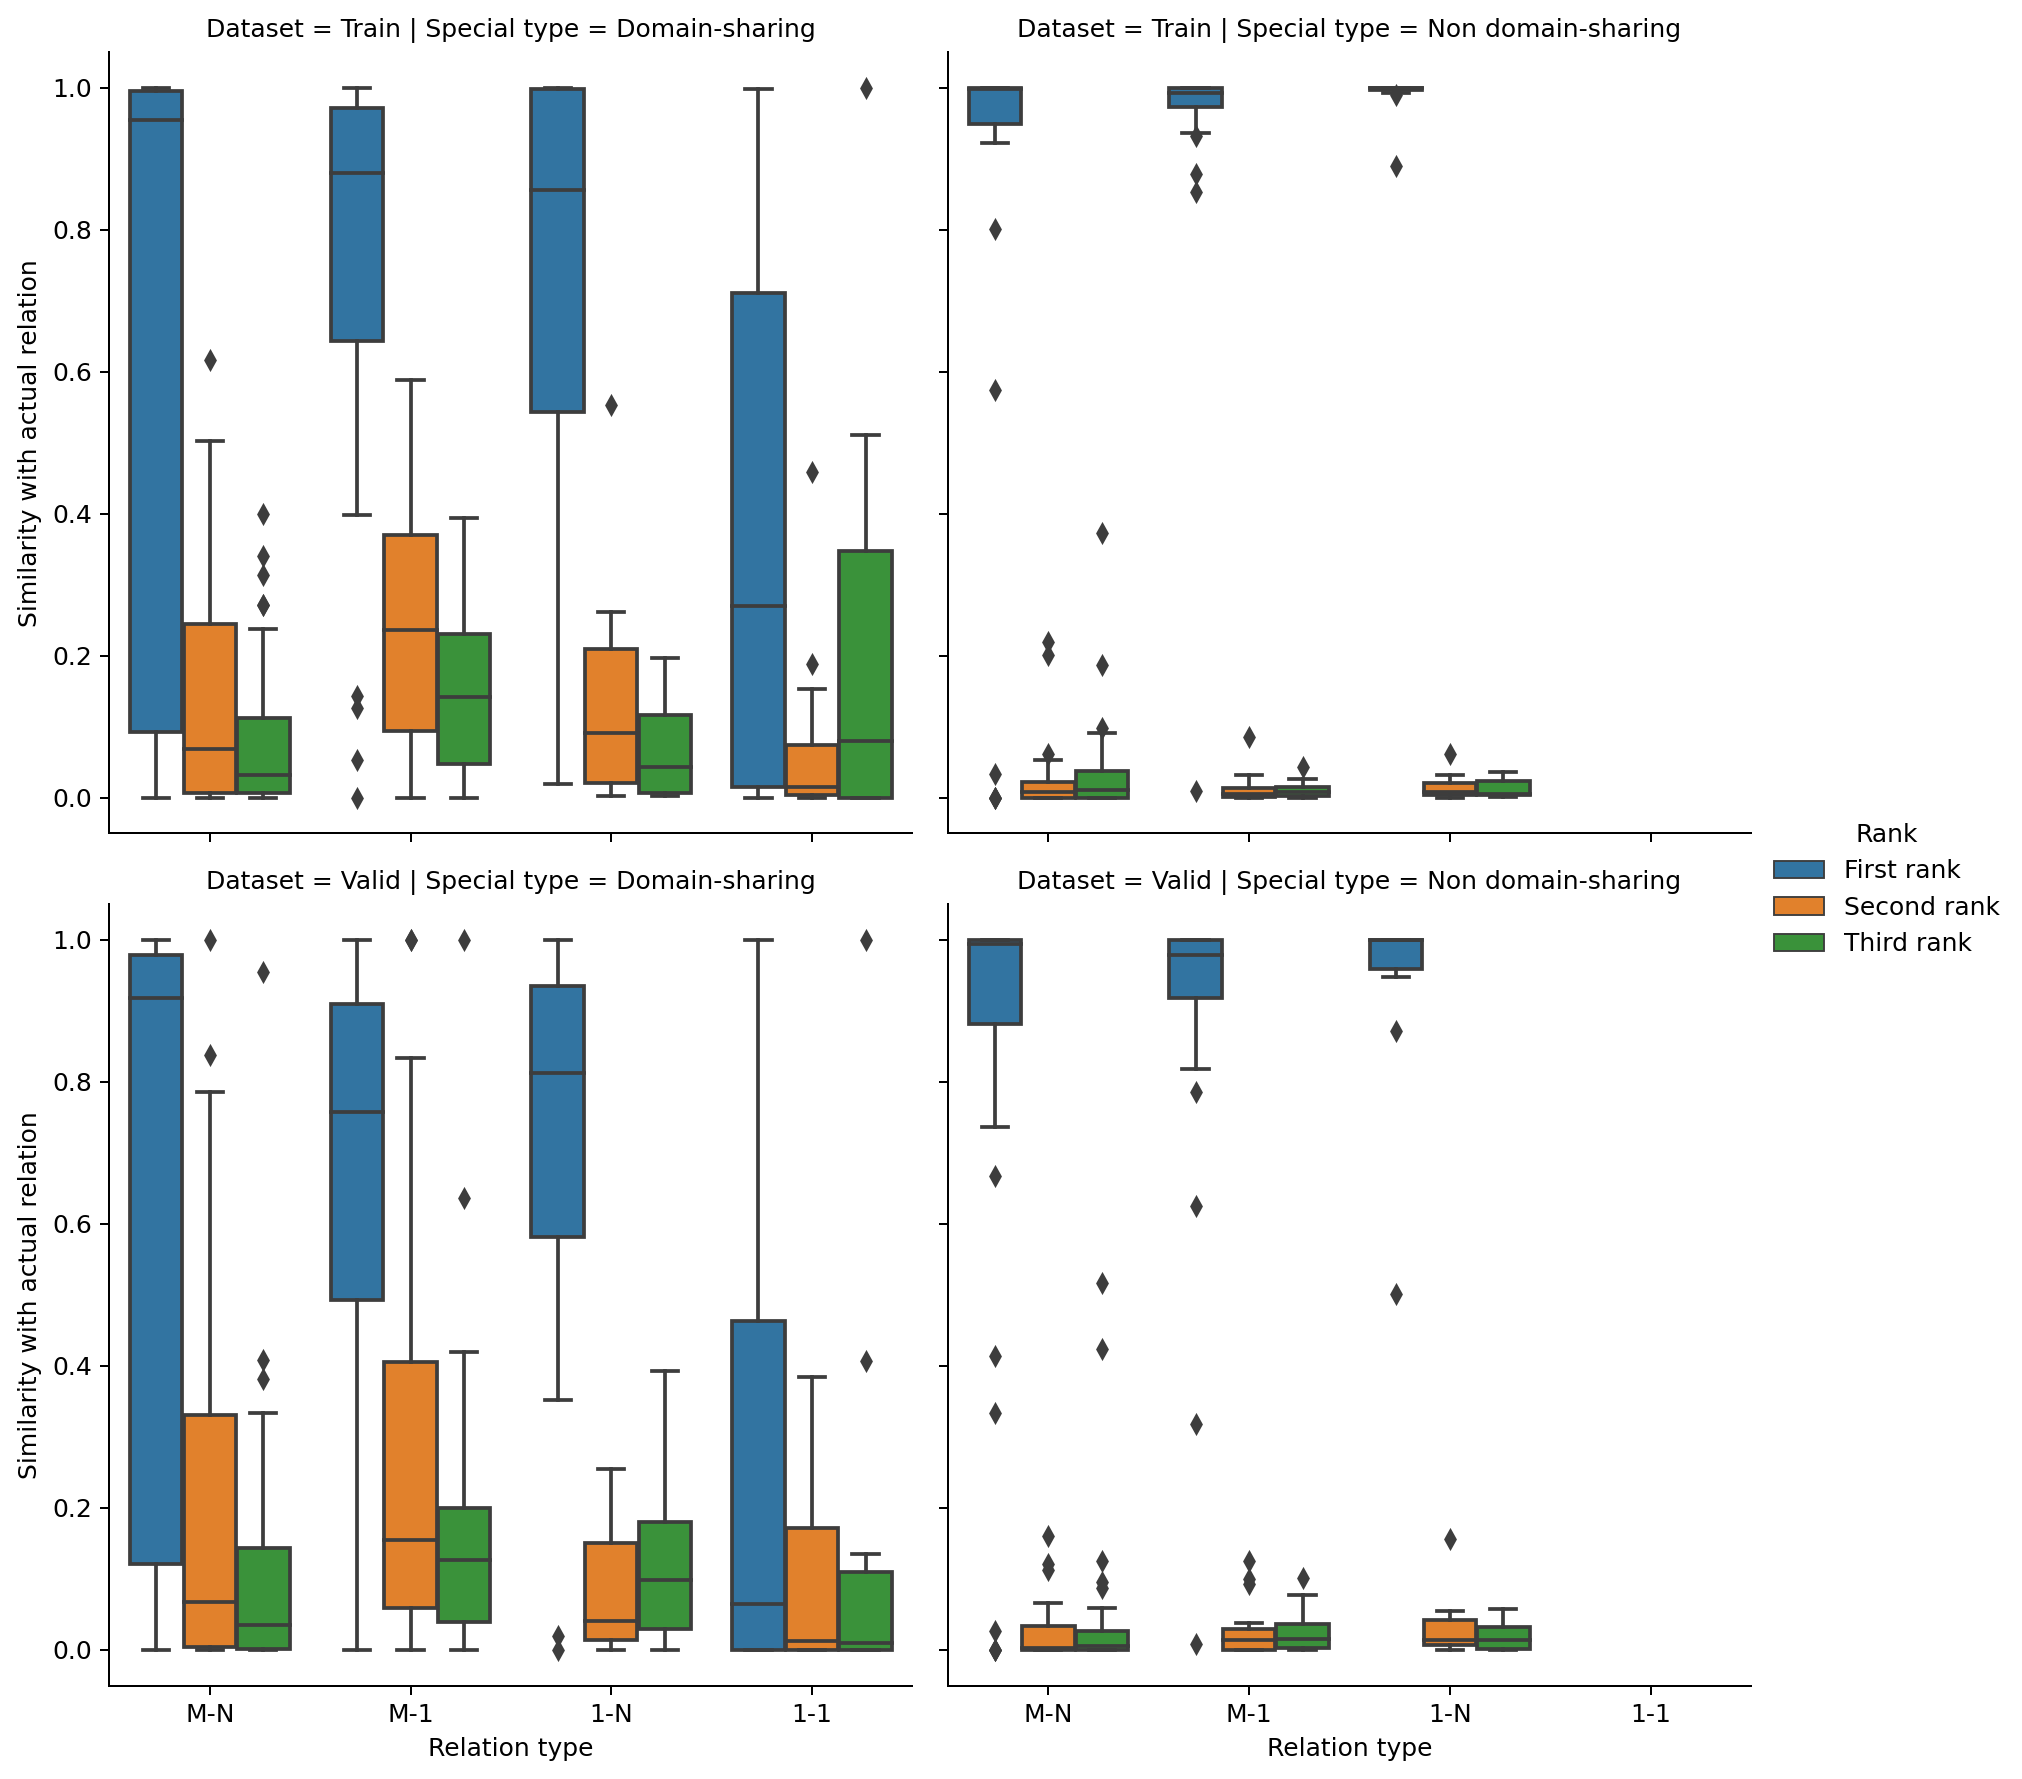
\includegraphics[width=\linewidth]{Images/jaccard_similarity (standard overall).png}
	\caption[Distribution of average similarity (standard overall)]{Distribution of average similarity between ranked relation and actual relation on validation and training data over relations for non domain-sharing and domain-sharing relations (standard overall model)}
	\label{fig:Jaccard similarity (standard overall)}
	\end{center}
\end{figure}

As shown in Figure \ref{fig:Jaccard similarity (standard overall)}, the first-rank relations for non domain-sharing relations are quite similar to the actual relation while the second and third rank relation are dissimilar to the true relation. Due to the characteristic of non domain-sharing relations, i.e, there does not exist another relation that has similar subject and object with this relation, the more similar to actual relation a relation is, the more they are the same. Therefore, by selecting the best-performance model on overall MRR, we can find a model could perform better on predicting non domain-sharing relation than the baseline model. 

However, Figure \ref{fig:Jaccard similarity (standard overall)} also highlights the limitation of standard overall model. We can see that there is a wide dispersion on similarity for domain-sharing relations, especially for first rank. Entity overall model could rank the similar relation to actual relation higher the for some of domain-sharing relations. However, generally speaking, the model still struggles on predicting the domain-sharing relation. Table \ref{tab:standard overall model example} illustrates some examples.

In sum, by selecting the best model on overall relation, we can find the model could achieve good MRRs for non domain-sharing relations without training from scratch or applying another training methods. However, it is not perfect, the model still struggles with some of domain-sharing relation, even though, we observed some improvement in predicting domain-sharing relation. 

% Please add the following required packages to your document preamble:
% \usepackage{booktabs}
% \usepackage{graphicx}
\begin{table}[!htbp]
\centering
\resizebox{\textwidth}{!}{%
\begin{tabular}{@{}lllcc@{}}
\toprule
\textbf{Subject} & \textbf{Relation} & \textbf{Object} & \textbf{Rank} & \textbf{Type} \\ \midrule
Demi Lovato & /celebrities/celebrity/celebrity\_friends./celebrities/friendship/friend & Taylor Swift & 14 & M-N \\
 & \quad /education/educational\_institution/campuses &  & 1 & 1-1 \\
 & \quad /education/educational\_institution\_campus/educational\_institution &  & 2 & 1-1 \\
 & \quad /location/hud\_county\_place/place &  & 3 & 1-1 \\ \midrule
My Name is Khan & /film/film/story\_by & Karan Johar & 3 & M-1 \\
 & \quad /film/film/written\_by &  & 1 & M-1 \\
 & \quad /film/film/produced\_by &  & 2 & M-1 \\
 & \quad /award/award\_winning\_work/awards\_won./award/award\_honor/award\_winner &  & 3 & M-1 \\ \midrule
Europe & /base/locations/continents/countries\_within & Poland & 3 & 1-N \\
 & \quad /education/educational\_institution/campuses &  & 1 & 1-1 \\
 & \quad /education/educational\_institution\_campus/educational\_institution &  & 2 & 1-1 \\
 & \quad /location/hud\_county\_place/place &  & 3 & 1-1 \\ \midrule
Austria & /base/aareas/schema/administrative\_area/capital & Vienna & 4 & 1-1 \\
 & \quad /education/educational\_institution\_campus/educational\_institution &  & 1 & 1-1 \\
 & \quad /education/educational\_institution/campuses &  & 2 & 1-1 \\
 & \quad /location/hud\_county\_place/place &  & 3 & 1-1 \\ \bottomrule
\end{tabular}%
}
\caption[Prediction examples from standard overall model.]{Prediction examples from standard overall model. The first relations on the top of each box are the true relations while the remain ones are the predicted relation.}
\label{tab:standard overall model example}
\end{table}



\section{Hybrid training objective with overall MRR}

As reported in Chapter \ref{chap:comparative_study}, to overcome the trade-off from selecting best model on overall MRR, we could re-train model with hybrid standard training objective and select the best model based on overall MRR. The hybrid overall model could achieve entity MRR of 34.6\% and relation MRR of 96.8\%.

\begin{figure}[!htbp]
	\begin{center}
	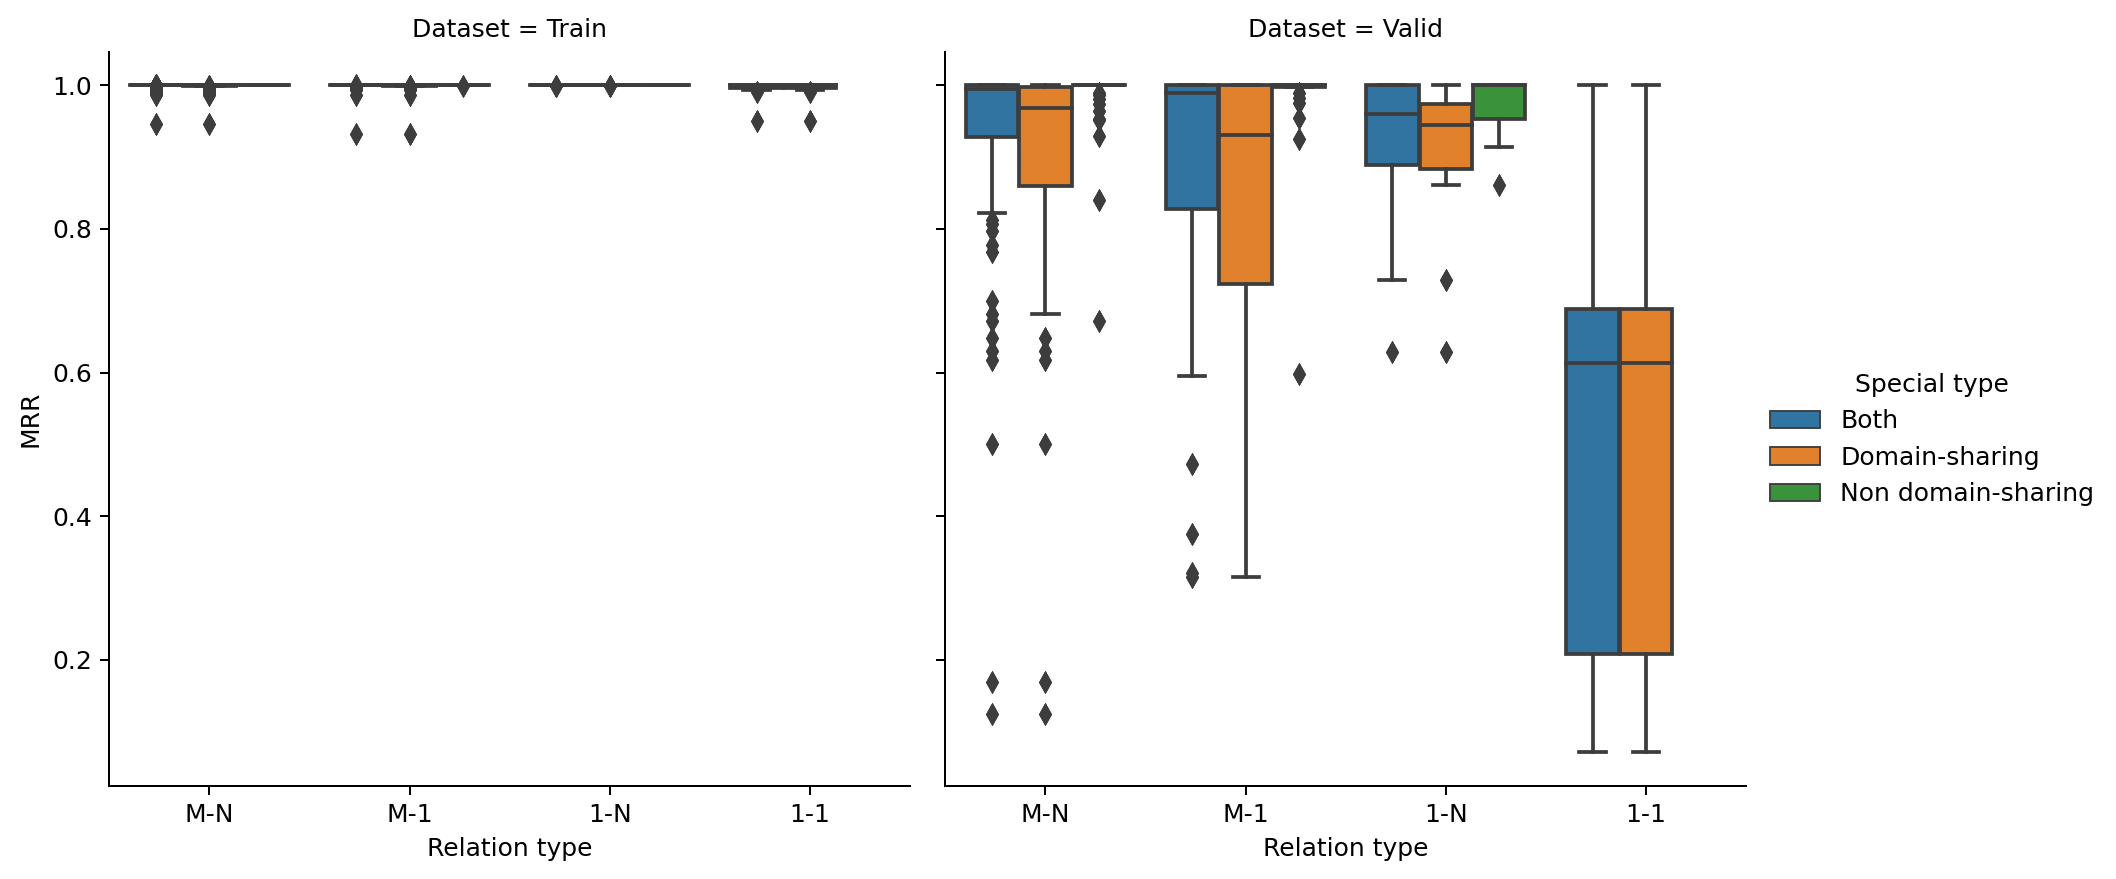
\includegraphics[width=\linewidth]{Images/MRR_relation_in_so_pairs (hybrid overall).png}
	\caption[Distribution of filtered relation MRR (hybrid overall)]{Distribution of filtered relation MRR on validation and training data over relations for for non domain-sharing and domain-sharing relations (hybrid overall model)}
	\label{fig:MRR relation in so pairs (hybrid overall)}
	\end{center}
\end{figure}

As illustrated in Figure \ref{fig:MRR relation in so pairs (hybrid overall)}, by training on hybrid training objective, undoubtedly, the best model could achieve significantly high MRRs on training dataset. Therefor, this in section, we mainly focus on the performance of hybrid overall model on validation dataset. 

It can be seen in Figure \ref{fig:MRR relation in so pairs (hybrid overall)}, most distributions of MRRs are not as dispersed as they were shown by other models and the median MRRs of all relation type are significantly higher than median MRRs from other models. This indicates that the hybrid overall model achieve high MRR consistently for most relation types. Furthermore, from Figure \ref{fig:Jaccard similarity (hybrid overall)}, we can clearly see that the model could rank the relation having similar domain with actual relation higher on both non domain-sharing and domain-sharing relations. Besides, we can also observed that the median of second rank is more higher than the third rank in domain-sharing relation which indicates that model now have ability to capture the domain that shared between domain-sharing relations


\begin{figure}[!htbp]
	\begin{center}
	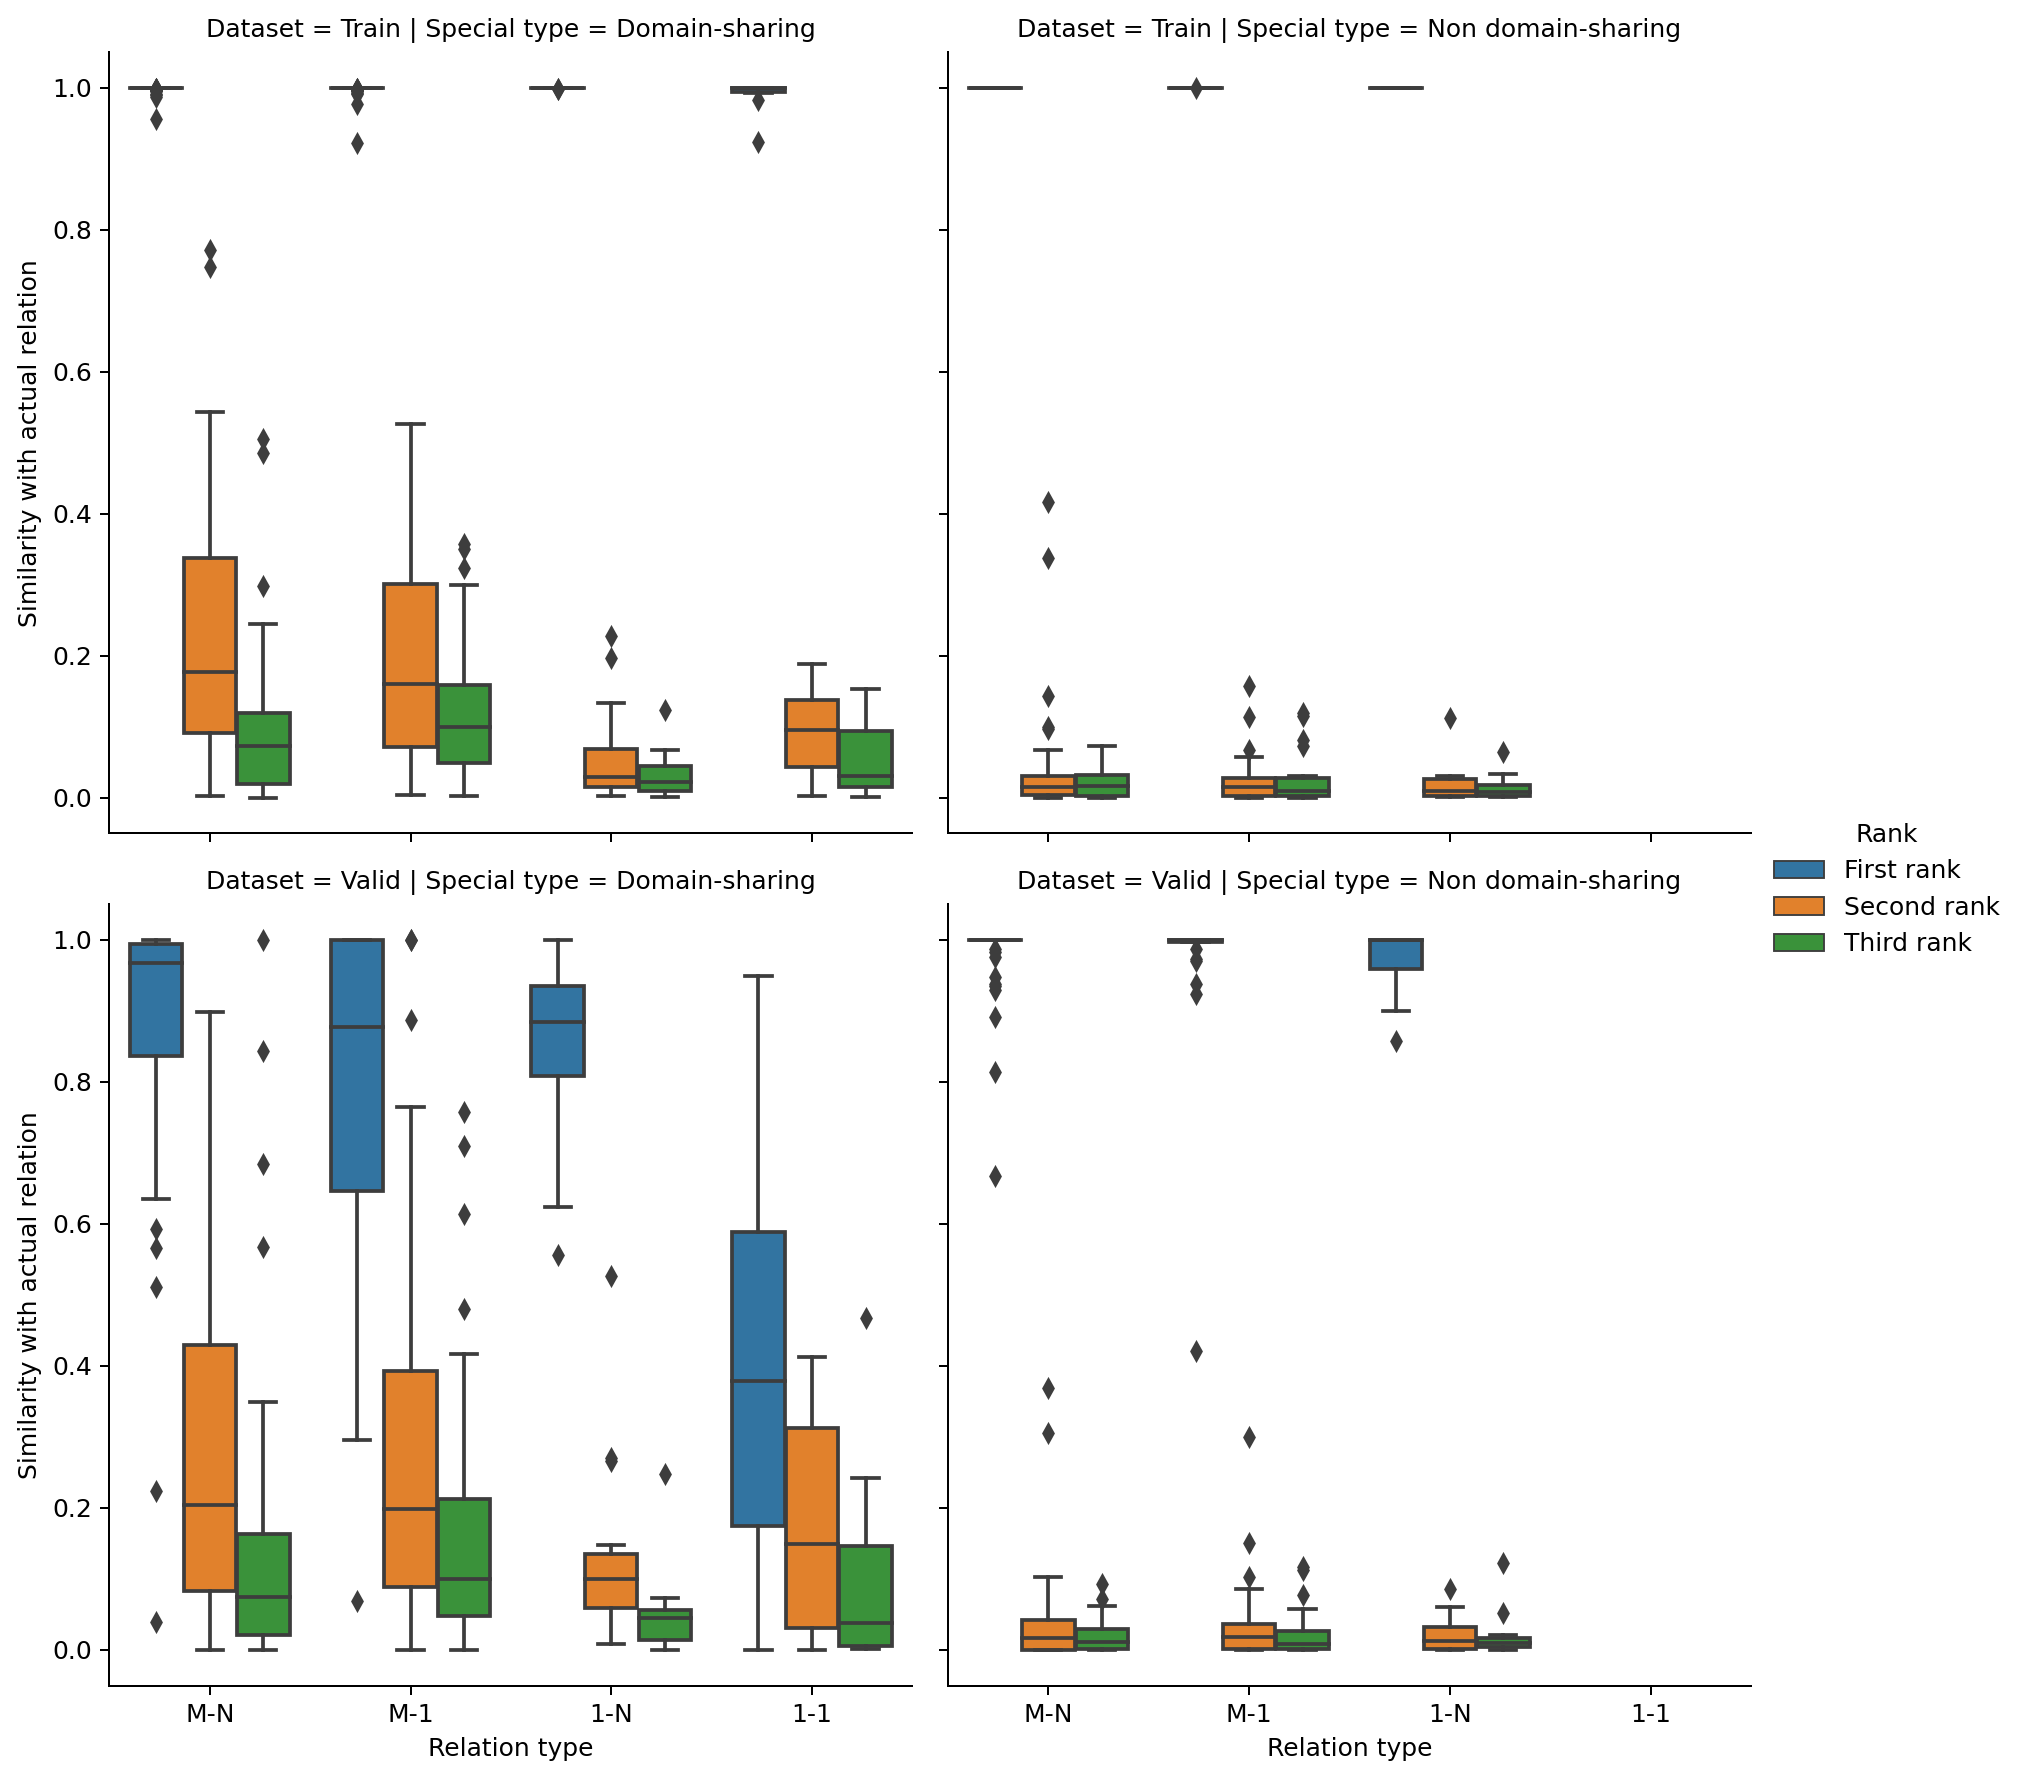
\includegraphics[width=\linewidth]{Images/jaccard_similarity (hybrid overall).png}
	\caption[Distribution of average similarity (hybrid overall)]{Distribution of average similarity between ranked relation and actual relation on validation and training data over relations for non domain-sharing and domain-sharing relations (hybrid overall model)}
	\label{fig:Jaccard similarity (hybrid overall)}
	\end{center}
\end{figure}


However, surprisingly, even we observed that the model can achieved high MRRs for 1-1 relation on training dataset in Figure \ref{fig:MRR relation in so pairs (hybrid overall)}, the hybrid overall model still showed a wide dispersion for 1-1 relations and median of MRR for 1-1 relation is just over 60\%. This could be a sign of overfitting in predicting 1-1 relations (Table \ref{tab:hybrid overall model example} illustrates some examples). 

% Please add the following required packages to your document preamble:
% \usepackage{booktabs}
% \usepackage{multirow}
% \usepackage{graphicx}
\begin{table}[!htbp]
\centering
\resizebox{\textwidth}{!}{%
\begin{tabular}{@{}lllcc@{}}
\toprule
\textbf{Subject} & \textbf{Relation} & \textbf{Object} & \textbf{Rank} & \textbf{Type} \\ \midrule
Singapore & /location/country/capital & Singapore & 3 & 1-1 \\
 & \quad /location/location/adjoin\_s./location/adjoining\_relationship/adjoins &  & 1 & M-N \\
 & \quad /military/military\_combatant/military\_conflicts./military/military\_combatant\_group/combatants &  & 2 & M-N \\
 & \quad /music/performance\_role/regular\_performances./music/group\_membership/role &  & 3 & M-N \\ \midrule
Syria & /sports/sports\_team\_location/teams & \multirow{4}{*}{\begin{tabular}[c]{@{}l@{}}Syria national\\  football team\end{tabular}} & 4 & 1-1 \\
 & \quad /people/person/profession &  & 1 & M-N \\
 & \quad /common/topic/webpage./common/webpage/category &  & 2 & M-1 \\
 & \quad /location/location/contains &  & 3 & M-N \\ \bottomrule
\end{tabular}%
}
\caption[Prediction examples from hybrid overall model.]{Prediction examples from hybrid overall model. The first relations on the top of each box are the true relations while the remain ones are the predicted relation.}
\label{tab:hybrid overall model example}
\end{table}


% lIMITATION could not answer the reason why we have the improvment







% As illustrated from Table \ref{tab:Top 3 predictions for each relation type}, the standard overall model could rank the relations which have similar type to actual relations higher than standard entity model. 

% \begin{figure}[!htbp]
% \centering
% \begin{subfigure}{\textwidth}
%     \centering
% 	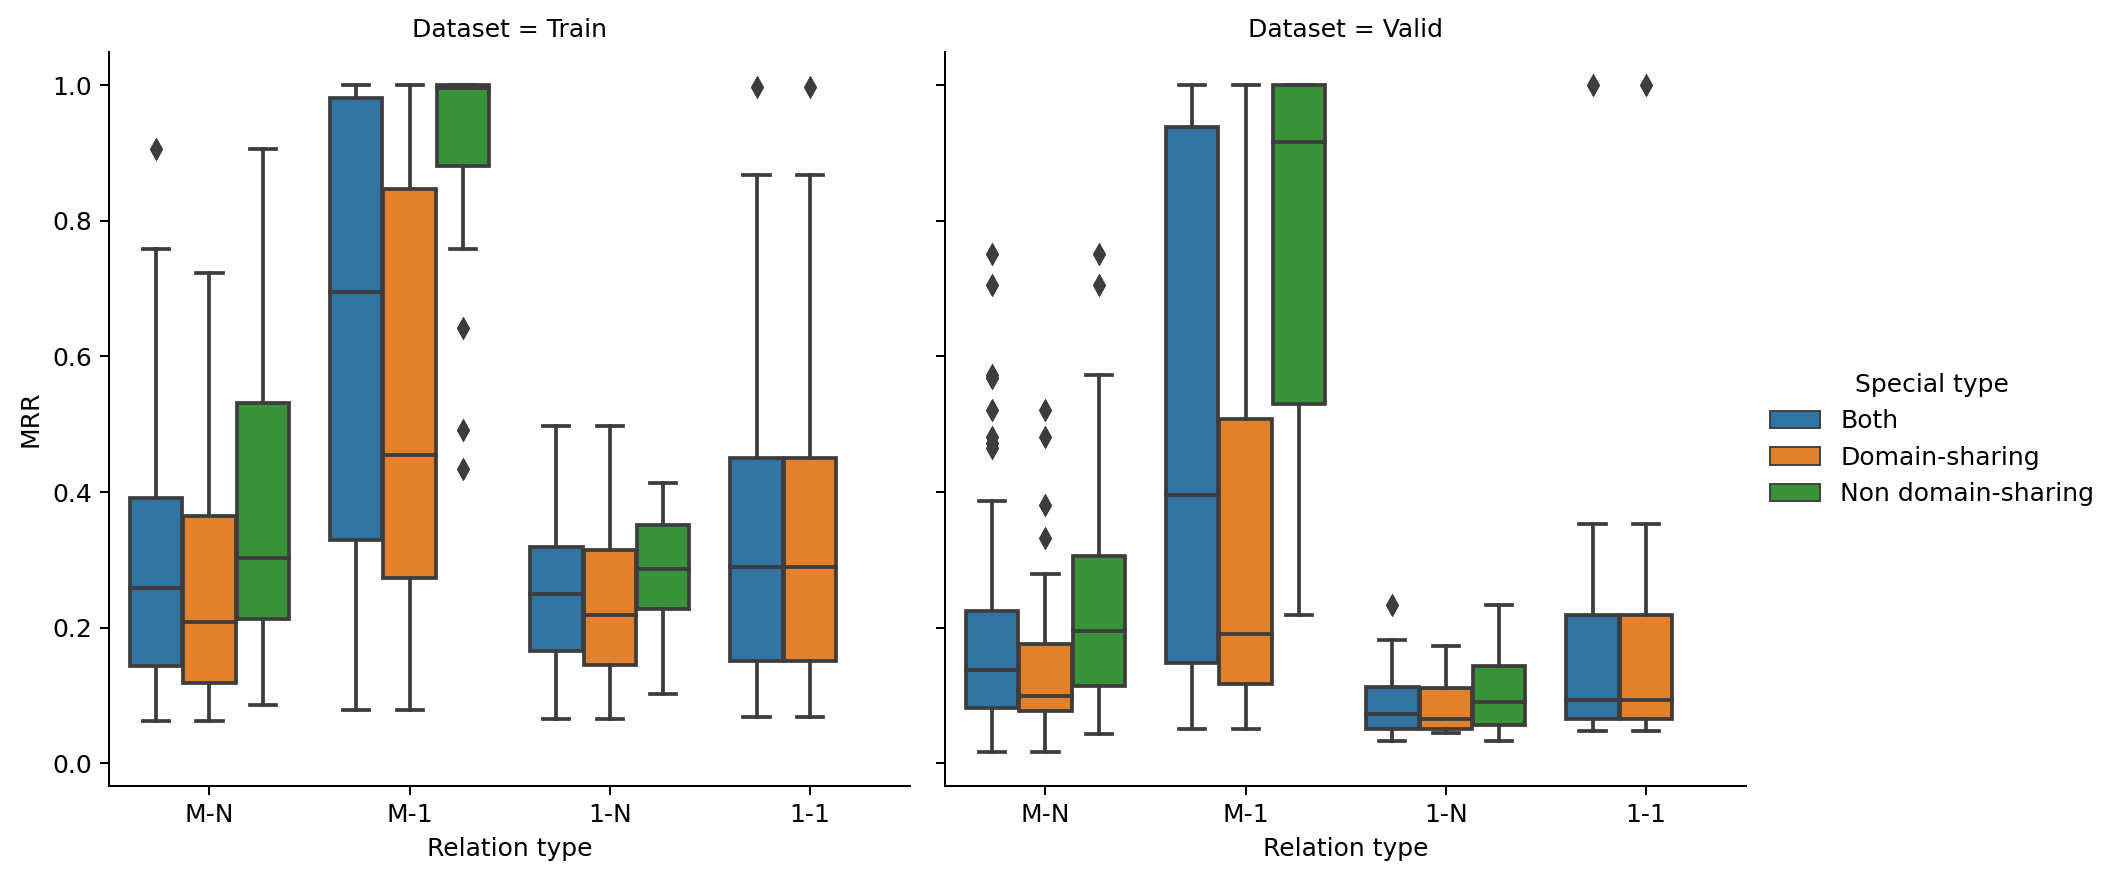
\includegraphics[width=\linewidth]{Images/MRR_relation_in_so_pairs (standard entity).png}
% 	\caption{(standard entity)}
% \end{subfigure}
% \vfill
% \begin{subfigure}{\textwidth}
%     \centering
%     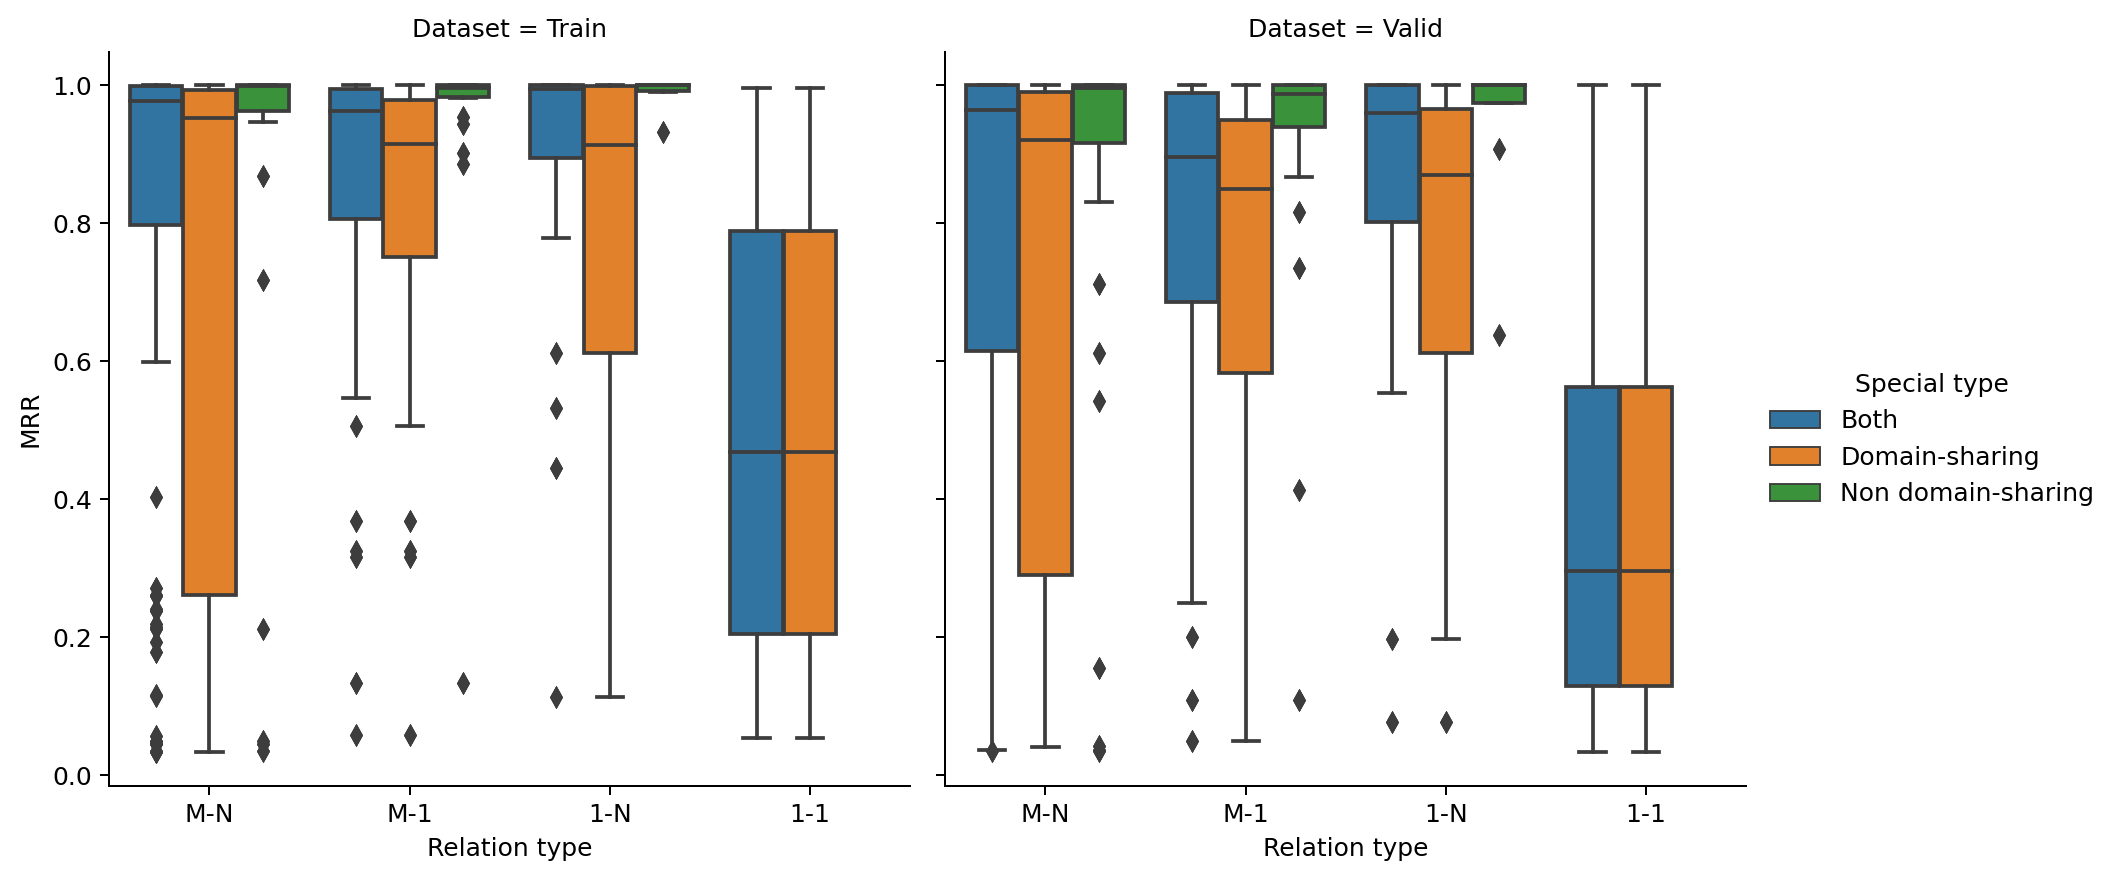
\includegraphics[width=\linewidth]{Images/MRR_relation_in_so_pairs (standard overall).png}
% 	\caption{(standard overall)}
% 	\label{fig:MRR relation in so pairs (standard overall)}
% \end{subfigure} 
% \caption{MRR of in non domain-sharing and domain-sharing relations}
% \label{fig:MRR relation in so pairs (standard overall)}
% \end{figure}







% \begin{figure}[!htbp]
% 	\begin{center}
% 	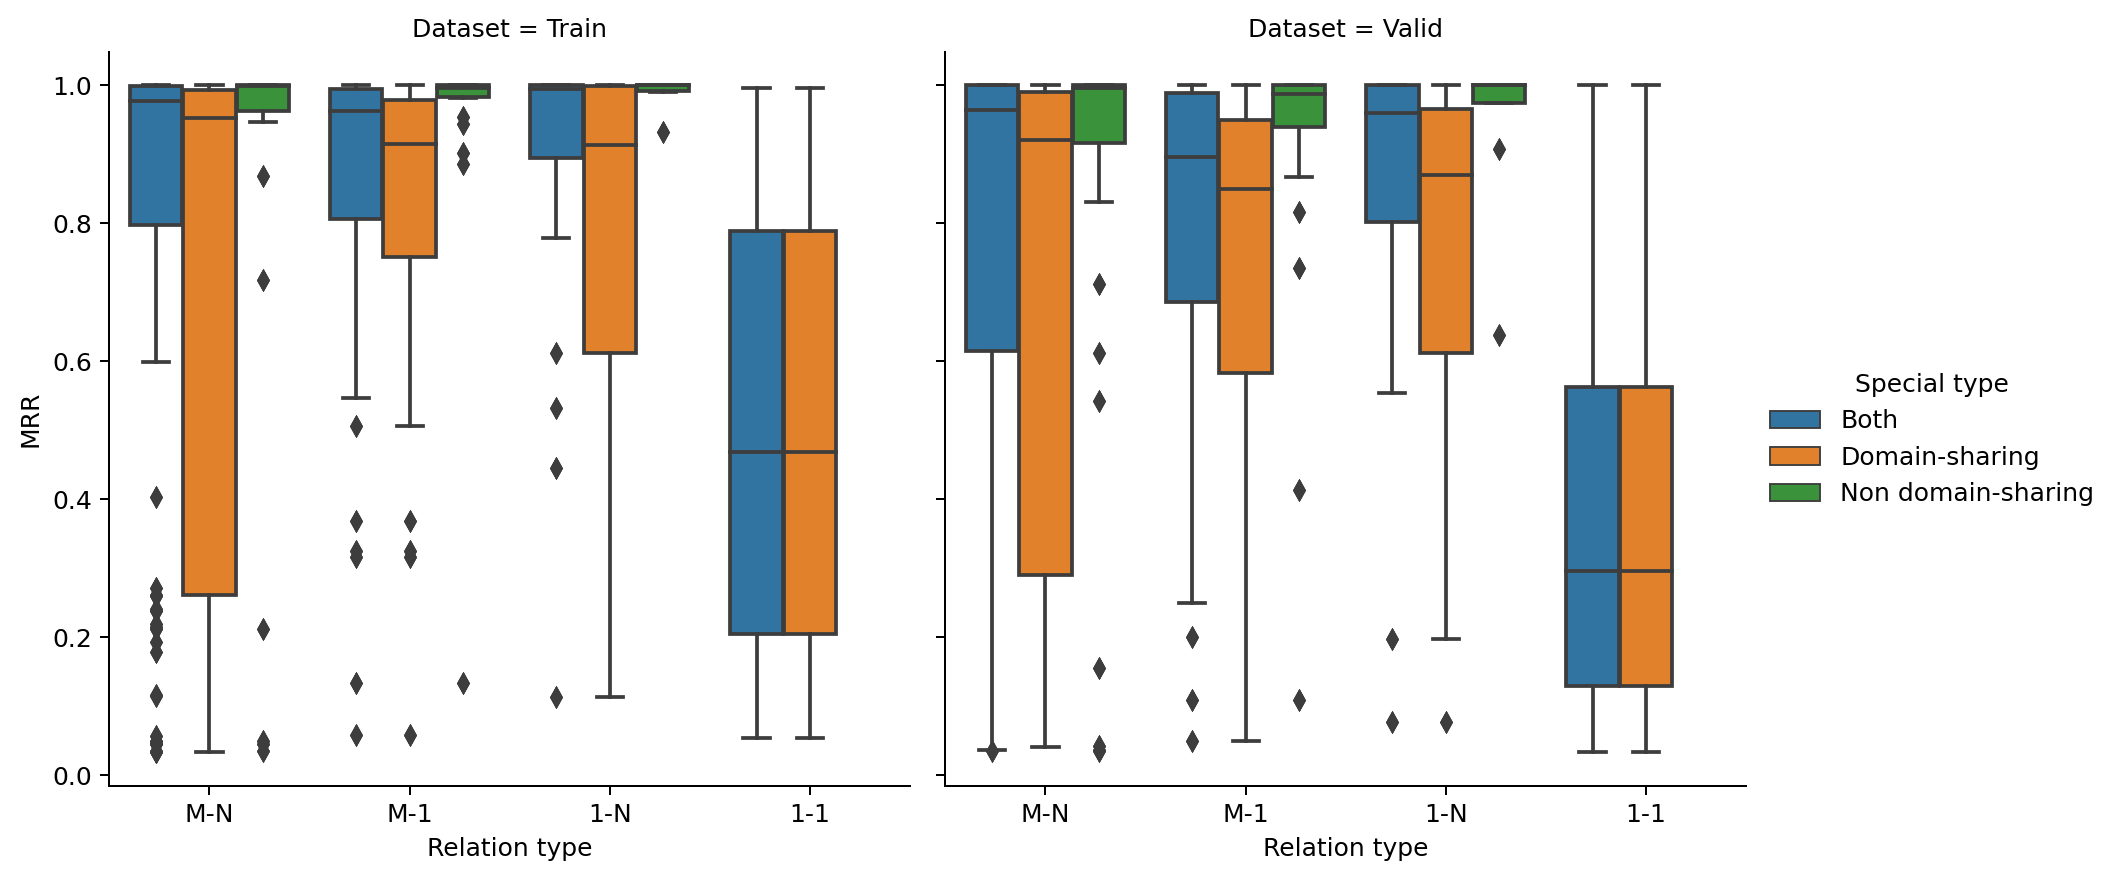
\includegraphics[width=\linewidth]{Images/MRR_relation_in_so_pairs (standard overall).png}
% 	\caption{MRR of in non domain-sharing and domain-sharing relations}
% 	\label{fig:MRR relation in so pairs (standard overall)}
% 	\end{center}
% \end{figure}















% % We found that, overall, the similarity between high-rank relations and the actual relations are quite low. However there is some noticeable point, the baseline model rank the quite similar relations higher for non-sharing domain relation than domain-sharing relation in both training and validation data. It means that, even the rank of true relation is not high, but the model could capture the meaning of relations for non-sharing domain relations better than sharing domain relations.    




% % Furthermore, to measure the domain similarity between actual relations $k$ and ranked relation $k'$, we calculate Jaccard similarity for (1) the pair of sets of subjects and sets of objects. 

% % % A place of birth is a lived place of a person, however, a lived place could not be implied to be a place of birth. 

% % %  could share a same domain (for subject is 0.42 and for object is 0.49), however, their meanings are not really the same.
 
% % % This is because the baseline model could not distinguish between M-N and M-1 relations (Table \ref{tab:MN to M1 examples}). 

% % Figure \ref{fig:Jaccard similarity MN} shows the distribution of similarity between the subject (object) set ranked relation and the subject (object) set of the actual relation. A subject (object) set of a specific relation $k$ is a set that for every entities in that set, there exist another object (subject) entity such that those three form a valid triple in a data. Let $\mathcal{E}_{s, k}$ denote the subject set of a specific relation $k$ and $\mathcal{E}_{o, k}$ denote the object set of a specific relation $k$.

% % % Formally, for example, given a triple $(i, k, j)$, model ranks a relation $k'$ at first rank and relation $k'$ have sets of corresponding subject entities $\mathcal{E}_{s, k'}$ and corresponding object entities $\mathcal{E}_{o, k'}$. Each entities in the set $\mathcal{E}_{s, k'}$ (or $\mathcal{E}_{o, k'}$) is a entity with the relation $k'$ that forms a valid triple in a data. 



% % % defined as $\mathcal{E}_{s, k'} = \{i'|i'\in\mathcal{E} \vee (i',k',*) \in \mathcal{D}\}$ and $\mathcal{E}_{o, k'} = \{j'|j'\in\mathcal{E} \vee (*,k',j') \in \mathcal{D}\}$. 


% % We chose Jaccard similarity to measure the similarity between two set of entities, for example subject sets, $J(\mathcal{E}_{s, k},\mathcal{E}_{s, k'}) = \frac{|\mathcal{E}_{s, k} \cap \mathcal{E}_{s, k'}|}{|\mathcal{E}_{s, k} \cup \mathcal{E}_{s, k'}|}$ where $k'$ is the ranked relation corresponding to the actual relation $k$. The similarity of domain between actual relation and ranked relation were calculated for all of triple. We averaged similarity by relation. 


% % \begin{figure}[!htbp]
% % \centering
% % \begin{subfigure}{\textwidth}
% %     \centering
% %     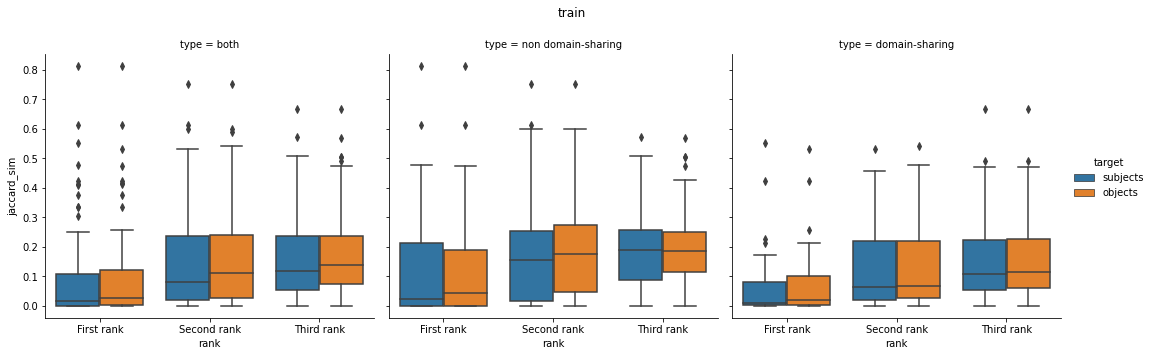
\includegraphics[width=\linewidth]{Images/jaccard_similarity_MN_train.png}
% %     \caption{Jaccard similarity MN (training data)}
% %     \label{fig:Jaccard similarity MN (train)}
% % \end{subfigure}
% % \vfill
% % \begin{subfigure}{\textwidth}
% %     \centering
% %     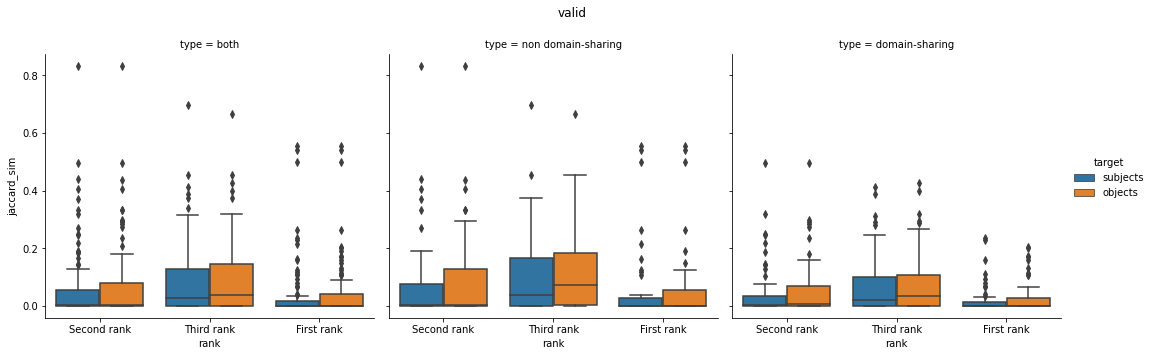
\includegraphics[width=\linewidth]{Images/jaccard_similarity_MN_valid.png}
% %     \caption{Jaccard similarity MN (validation data)}
% %     \label{fig:Jaccard similarity MN (valid)}
% % \end{subfigure} 
% % \caption{Jaccard similarity MN}
% % \label{fig:Jaccard similarity MN}
% % \end{figure}





% % An interesting observation is that baseline model ranked those relations that do not share similar domain with the true relation higher when the actual relations are sharing domain relations. While for those true relations that are non-sharing domain relation, model could rank the relation having same domain higher which is the true relation. Therefore, as shown in Figure \ref{fig:MRR of MN relation in so pairs}, standard model selected on entity MRR achieve higher MRRs (on average) in non-sharing domain relations than in sharing domain relations on both validation and training data.



% % M-1 and M-N but M-N have the same domain for subject and object but the meaning is not really the same, for example "lived place" and "place of birth", a place of birth is a lived place of a person, but, a lived place could not be implied to be a place of birth. 








% \noindent\textbf{1-N relations vs M-1 relations.}  The main different between two types is that the subject of 1-N relation can be associated with many different object entities while subject in M-1 relation can only be associated with 1 object entity. For example, in 1-N "Countries within" relation, Asia contains 48 countries such as Vietnam, Laos, Cambodia, while in M-1 "Administrative division of" relation, one city can belong to one and only one country e.g., Munich is city of Germany and only belongs to Germany. However, as can be seen from Table \ref{tab:Top 3 predictions for each relation type}, given a 1-N relation prediction query $(s,?,o)$, model trained with standard training objective gives high rank to M-1 relations most of the time. Table \ref{tab:1N to M1 examples} shows two examples of prediction.


% \begin{table}[!htbp]
% \centering
% \resizebox{\textwidth}{!}{%
% \begin{tabular}{@{}llllllcl@{}}
% \toprule
% \textbf{Subject} & \textbf{Relation} & \textbf{Subject} & \textbf{Rank Relation} & \textbf{Type relation} & \textbf{Predicted} & \textbf{Rank} & \textbf{Type prediction} \\ \midrule
% Robert Rodriguez & Director of film & Sin City & 7 & 1-N & Producer type & 1 & M-1 \\
%  &  &  &  &  & GDP region currency & 2 & M-1 \\
%  &  &  &  &  & GDP per capita currency & 3 & M-1 \\ \midrule
% Euro & Countries within & Poland & 9 & 1-N & First level of administrative division of & 1 & M-1 \\
%  &  &  &  &  & Administrative division of & 2 & M-1 \\
%  &  &  &  &  & Location in & 3 & M-1 \\ \bottomrule
% \end{tabular}%
% }
% \caption{}
% \label{tab:1N to M1 examples}
% \end{table}

% Additionally, investigating the first top 3 predicted relations revealed that the meaning of predicted relations were not quite close to the true relations (examples in Tables \ref{tab:1N to M1 examples} and \ref{tab:MN to M1 examples}). One reason is that, because the true relations always existed in the queries when training with standard objective, thus, the baseline model needs to learn only the interaction of a relation with given subjects or objects. Therefore, those relations that share the same subject and object domains together, have similar vector representations. The Figure 

% However, some relations do not share the same subject and object domain but are related to each other. Training with hybrid model can capture those relation.

% Figure \ref{fig:similarity distribution} shows the cosine similarity between relations. As can be seen, baseline model considers most of relations to be different to each other.   

% \begin{figure}[!htbp]
% 	\begin{center}
% 	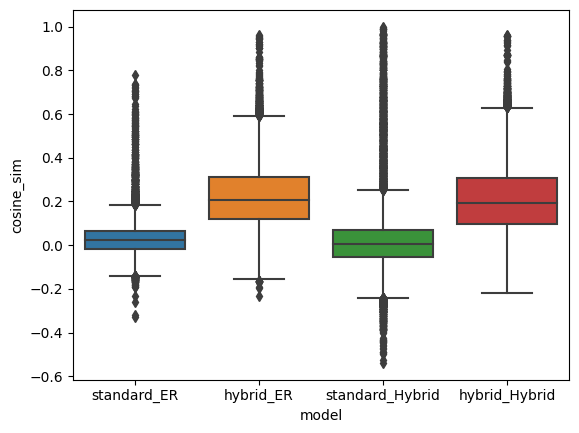
\includegraphics[width=0.8\linewidth]{Images/similarity_dist.png}
% 	\caption{Relation similarity distribution}
% 	\label{fig:similarity distribution}
% 	\end{center}
% \end{figure}

% Investigating the outlier similarity show that Similary (Table \ref{tab:so pairs})

% \begin{figure}[!htbp]
% 	\begin{center}
% 	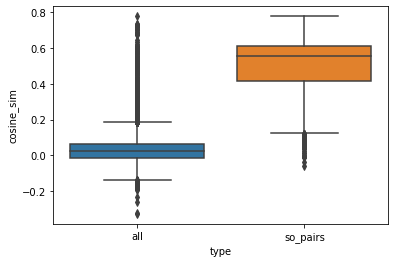
\includegraphics[width=0.8\linewidth]{Images/so_similarity_baseline.png}
% 	\caption{so similarity baseline}
% 	\label{fig:so_similarity_baseline}
% 	\end{center}
% \end{figure}



% \section{Model Selection: overall MRR}

% By selecting model on overall MRR, we compromised between entity MRR and relation MRR therefore, the performance on relation prediction increased but the performance on entity ranking reduced and there were too many outliers. Furthermore, the MRR distribution of 1-1 relation and M-N are quite dispersed.

% The 

% Now model could distinguish the domain, but, the model still not distinguish the meaning 

% \section{Hybrid training objective}